\section{Planning and Control}
\label{sec:processing_and_control}
This section covers our approach to preplanning motion waypoints for the soft robot and controlling the manipulator along those points. We cover existing procedures reused within the system, and detail the system's new architecture of for performing autonomous grasp-and-place tasks, including its main component, the Grasp Object Planner.

\subsection{Existing Procedures}
The forward kinematics algorithm \texttt{forwKin()}, which we employ in this work, assumes piece-wise constant curvature according to \cite{webster2010design}. 
This algorithm was experimentally validated for the soft planar arm in \cite{marchese2014design}.
In order to uniquely fit a configuration representation to measured endpoint data in real-time, we use a previously developed single segment inverse kinematics algorithm \cite{marchese2014design} and refer to it in this work as \texttt{singSegInvKin()}.
The inputs to this block are the start and endpoint measurements in $\mathbb{R}^2$: $\mathbf{E}_n \; \forall n  = 1..N$, where $N$ is the number of segments composing the arm.
The outputs from this block are the representations of the measured manipulator configuration: $\boldsymbol{\kappa}_{\textrm{meas}}$ and $\mathbf{L}_{\textrm{meas}}$.
\rkk{Each segment of the manipulator is described by its measured curvature $\kappa_{\textrm{meas}}$ and its segment length $L_{\textrm{meas}}$}.
This work expands on the previously developed cascaded closed-loop curvature controller, whose input is target curvatures $\boldsymbol{\kappa}_{\textrm{target}}$ and whose output is the controlled adjustment of a fluidic drive cylinder array to resolve the error between $\boldsymbol{\kappa}_{\textrm{target}}$ and $\boldsymbol{\kappa}_{\textrm{meas}}$.
In this work we refer to it as the \texttt{curvatureController()}.

The planning algorithm presented in \cite{marchese2014whole} was developed to plan the motion of a soft arm  without gripper through a confined environment. 
The optimization constraints and state machine setup in that work is significantly different and not applicable to the grasping shown here. 
Therefore, a new planner is presented in the following section.

\subsection{Autonomous Grasp-and-Place System}
\label{subsec:grasp-place-planner}
The robotic manipulation system is capable of autonomously performing grasp-and-place operations. 
A state flow diagram describing its sensing, planning and executions states is given in Fig. \ref{fig:grasp-and-place-planner}. 
A motion tracker constantly captures the position of the object and passes it along to a routine, which checks for the object to settle.
\rkk{We consider the object to have settled if it has not moved by more than a small $\epsilon$ for 2\unit{s}}.
After it has settled, the Grasp Object Planner receives the coordinates and radius of the settled object and together with the current curvature values of the arm and gripper, it solves a series of constrained nonlinear optimization problems to generate end-effector poses approaching the object.
Those end-effector poses are essentially waypoints for an optimized path the robot arm should take to get to the final position without the risk of pushing away the object before the gripper arrives there. 
Forcing the arm controller to follow those intermediate waypoints ensures that the arm moves to the object while its null space maintains a convex shape, bending away from the object. 
Furthermore, it allows the arm to move in smaller portions, decreasing the risk of large overshoots due to slip-stick friction between the roller supports and the ground.
This planner is described in more detail in Section~\ref{subsec:grasp_planner}.

\begin{figure}[!htb]
\centering
   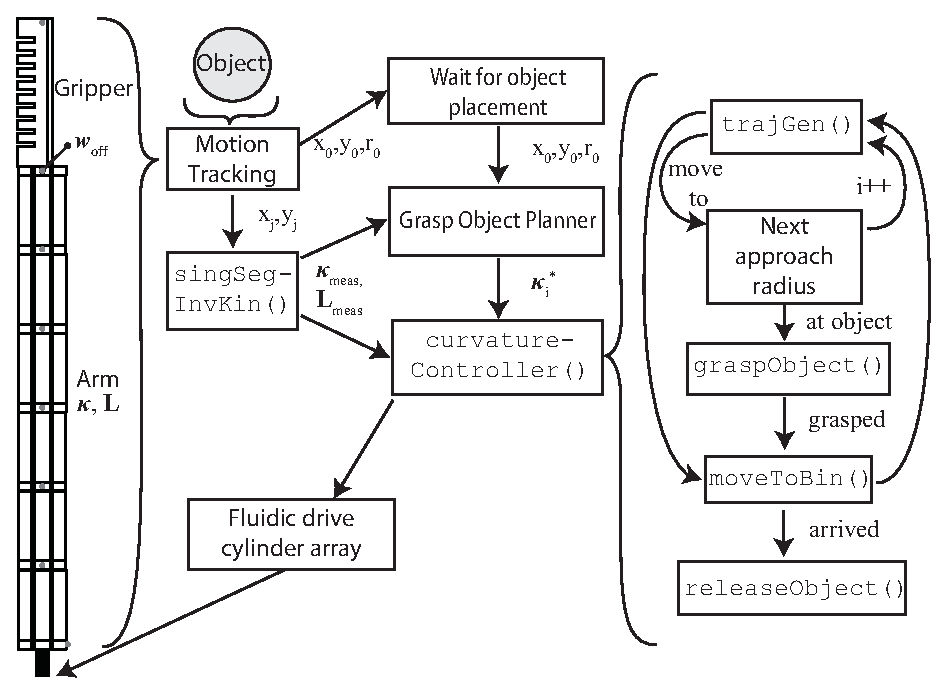
\includegraphics[width=0.95\columnwidth]{Figures/processing_control/grasp_place_planner.eps}
   \caption{State flow diagram of the grasp-and-place planner developed for the autonomous grasp-and-place operation of the manipulator. This diagram describes essentially the flow of information from the motion tracking system to the discrete hardware.}
   \label{fig:grasp-and-place-planner}
\end{figure}

The Grasp Object Planner passes the approach configurations $\boldsymbol{\kappa}_i^*$ of the arm to the \texttt{curvatureController()} for execution in real-time.
The controller receives measured curvatures $\boldsymbol{\kappa}_{meas}$ and lengths $\boldsymbol{L}_{meas}$ at an update rate of $100\unit{Hz}$ from the recursively called \texttt{singSegInvKin()} and uses these to successively control the arm to every intermediate configuration $\boldsymbol{\kappa}_i^*$.
During the arm initialization, the new curvature controller performs a pre-pressurization of both lateral channels. 
This is only done for the two segments closest to the root of the arm in order to stiffen them and shorten their response time constant.  
To allow for smoother transitions between each configuration $\boldsymbol{\kappa}_i^*$, we also added a trajectory generation procedure \texttt{trajGen()} to the new curvature controller. It generates in real-time for each individual degree-of-freedom velocity profiles with acceleration and velocity constraints.
These profiles allow real-time interpolation between the approach configurations of the arm and avoid overshooting at the next target configuration.
When the arm has arrived at the object, the curvature controller initiates \texttt{graspObject()}.
After encapsulating the object, \texttt{moveToBin()} requests \texttt{trajGen()} for another trajectory from the current pose to a pre-defined bin location.
After the manipulator has arrived at the bin location, the procedure \texttt{releaseObject()} causes the gripper to open and release the object.

\subsection{Grasp Object Planner}
\label{subsec:grasp_planner}
A fundamental component of the grasp-and-place system is its ability to plan a feasible approach motion to the object.
That is, given the location $\left(x_o, \, y_o\right)$ and radius $r_o$ of a round object as well as the manipulator's current configuration $\boldsymbol{\kappa}_{\textrm{meas}}$ \rkk{and segment lengths $\mathbf{L}_{\textrm{meas}}$}, we determine a series of locally optimal manipulator configurations $\boldsymbol{\kappa}_i^* \; \forall i \, = 1.. numMoves$ that will, if sequentially achieved, bring the manipulator gradually closer to the object while any part of the arm is not touching the object.

We refer to these as approach configurations.
The process for determining these approach configurations is detailed in the \texttt{planGrasp()} procedure within the Grasp Object Planner, see Algorithm \ref{alg:planGrasp}.
The planner is visualized in Figure \ref{fig:planGrasp}.
In short, we define a series of approach radii $r_{a_i} \;  \forall i\, = 1.. numMoves$ that define concentric circles shrinking from the manipulator's starting tip pose towards the center of the object.
Given actuator limits, we then search for a series of feasible manipulator configurations $\boldsymbol{\kappa}_i^*$ that will place the robot's end-effector on these \rkk{green} circles, parameterized by $r_a$ and $\phi$, while minimizing manipulator deformation.

\begin{figure}[htpb]
\centering
   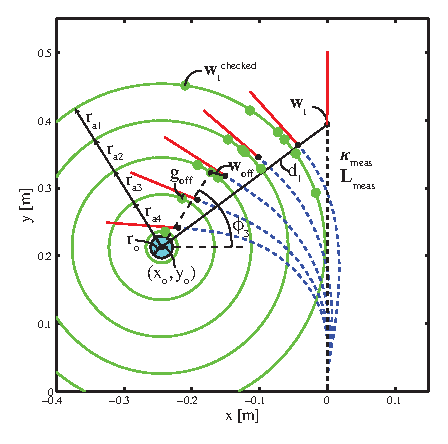
\includegraphics[width=0.85\columnwidth, trim = 0mm 0mm 5mm 5mm, clip]{Figures/processing_control/grasp_object_planner.eps}
   \caption{Visualization of the Grasp Object Planner. Concentric approach circles are shown in \emph{green} and are centered about the object shown in \emph{cyan}. The locally optimal approach configurations are shown in \emph{blue} and the gripper is shown in \emph{red}. The initially measured manipulator configuration is shown in black.}
   \label{fig:planGrasp}
\end{figure}

\begin{algorithm}[!htbp]
\begin{small}
  \SetAlgoLined\DontPrintSemicolon
  \KwIn{
  $\boldsymbol{\kappa}_{\textrm{meas}}$, $\mathbf{L}_{\textrm{meas}}$ $\gets$ measured arm configuration \;
  $\boldsymbol{\kappa}_{\textrm{off}}$ $\gets$ \rkk{measured manipulator} configuration at start \;
  $g_{\textrm{off}}$ $\gets$ gripper offset normal to end-effector\;
  $x_o$, $y_o$, $r_o$ $\gets$ object center coordinates and radius \;
  $N$ $\gets$ number of manipulator segments}
  \SetKwFunction{planGrasp}{planGrasp}
  \SetKwFunction{findOptimalConfig}{findOptimalConfig}
  \SetKwFunction{forwKin}{forwKin}
  \SetKwProg{myproc}{Procedure}{}{}
  \myproc{\planGrasp{}}{
  $\mathbf{w}_t \gets \forwKin \left( \boldsymbol{\kappa}_{\textrm{meas}}, \, \mathbf{L}_{\textrm{meas}}, \, N, \, L_N \right)$. \;
  $d_1 \gets \| \left[ x_o, \, y_o \right]^{\textrm{T}} \, - \, \mathbf{w}_t \|$. \;
  $d_2 \gets d_1 - r_o - g_{\textrm{off}}$. \;
  $numMoves \gets \lfloor \frac{d_2}{\Delta d} \rfloor$. \;
  $i$ = 0. \;
  \Repeat{$i$ = $numMoves$}{
    $i$ = $i \, + \, 1$ \;
    $r_{a_i} \gets d_1 \, - \, i\,\frac{d_2}{numMoves}$. \;
    $\boldsymbol{\kappa}_i^* \gets$ \findOptimalConfig{$r_{a_i}$}\;
  }
  \KwRet{$\boldsymbol{\kappa}_i^* \quad \forall i \, = 1.. numMoves$} \;}{}
  \setcounter{AlgoLine}{0}
  \SetKwProg{myproc}{Procedure}{}{}
  \myproc{\findOptimalConfig{$r_a$}}{
  $\begin{aligned}
    & \boldsymbol{\kappa}^* \, \gets \, \underset{\phi, \, \boldsymbol{\kappa}}{\text{min}}
    & & \mathbf{R} \, \left( \boldsymbol{\kappa} \, - \, \boldsymbol{\kappa}_{\textrm{off}} \right)^2. \\
    & \text{subject to}
    & &  \mathbf{w}_t \gets \begin{bmatrix} x_o \, + \, r \, \cos{\phi} \\ y_o \, + \, r \, \sin{\phi} \\ \phi \, + \, \frac{\pi}{2} \end{bmatrix}. \\
    & & & \mathbf{f} \gets \forwKin\left( \boldsymbol{\kappa}, \, \mathbf{L}, \, N, \, L_N \right). \\
    & & & \mathbf{w}_t - \mathbf{w}_{\textrm{off}}\left(r_o, \, \phi \right) - \mathbf{f} \, = \, \mathbf{0}. \\
    & & & \kappa_{n}^{\text{min}} \leq \kappa_n \leq \kappa_{n}^{\text{max}} \quad \forall \, n = 1 \, .. \,N. \\
    \end{aligned}$ \;
  \KwRet{$\boldsymbol{\kappa}^*$} \; }
  \setcounter{AlgoLine}{0}
  \SetKwProg{myproc}{Procedure}{}{}
  \myproc{\forwKin{$\boldsymbol{\kappa}$, $\mathbf{L}$, $i$, $s$ }}{
  \KwIn{$\boldsymbol{\kappa}$, $\mathbf{L}$, $i$ the segment of interest index, $s$ the arc length along the indexed segment}
  \eIf{$i = 0$}{
        $\theta_{i}(0) \gets \theta_0(0)$. \;
        $x_{i}(0) \gets 0$.\;
        $y_{i}(0) \gets 0$.\; }
    {
        $\left[ x_{i}(0), \, y_{i}(0), \, \theta_{i}(0) \right] \gets \forwKin \left(\boldsymbol{\kappa}, \, \mathbf{L}, \, i-1, \, L_{i-1} \right)$.\;
    }
    $\theta \gets \theta_{i}(0) + k_i s$. \;
    $x \gets x_{i}(0) + \frac{\sin{\theta}}{k_i} - \frac{\sin{\theta_{i}(0)}}{k_i}$. \;
    $y \gets y_{i}(0) - \frac{\cos{\theta}}{k_i} + \frac{\cos{\theta_{i}(0)}}{k_i}$. \;
  \KwRet{$\left[ x, \, y, \, \theta \right]^{\mathrm{T}}$ or $\left[ x, \, y \right]^{\mathrm{T}}$}}
  \caption{Grasp Object Planner}
  \label{alg:planGrasp}
\end{small}

\end{algorithm}

The procedure first determines the manipulator's current tip pose $\mathbf{w}_t$ and the Euclidean distance $d_1$ between the tip and the object's center. 
\rkk{The arc length input to the arm's forward kinematics is the $N$-th element of the segment lengths $\mathbf{L}_{\textrm{meas}}$.}
Next, considering the object's radius $r_o$ and the gripper normal offset $\mathbf{g}_{\textrm{off}}$, the minimal tip transit distance $d_2$ is calculated. 
\rkk{The end effector offset $\mathbf{w}_{\textrm{off}}$ describes the distance from the root of the gripper, to an offset point close to the lower end of the gripper's palm. It is visualized in the top left corner of Fig.~\ref{fig:grasp-and-place-planner}.}
\rkk{The length} $\mathbf{g}_{\textrm{off}}$ represents the component of the end effector offset $\mathbf{w}_{\textrm{off}}$, which is normal to the end effector orientation. 
Also, the number of approach configurations $numMoves$ is determined as $\lfloor \frac{d_2}{\Delta d} \rfloor$, where $\Delta d$ is an allowable incremental distance. 
Using these parameters, approach radii $r_a$ are iteratively calculated and their corresponding locally optimal configurations are found using the \texttt{findOptimalConfig($r_a$)} procedure. 
This process is posed as a nonlinear optimization. 
Here, the objective function represents the summation of independently weighted manipulator curvatures and the constraints force the manipulator's tip to lie on and to be tangent to the approach circle. 
This process leverages the arm's forward kinematics \texttt{forwKin()} defined in \cite{marchese2014design} and reproduced in Algorithm \ref{alg:planGrasp} for convenience. 

